%!TEX root = paper.tex
\section{Numerical Evaluation}
\label{sec:numerical}
We implement\footnote{\url{https://github.com/fmetzger/ggsn-simulation/}} the models introduced in \refsec{model} using a \gls{DES} with the SimPy \cite{simpy} package as foundation.
To be in line with the measurement data we consider a simulation time of seven days for all simulation scenarios, with a transient phase of 60 minutes accounted for. Ten replications of each scenario were performed.
All error bars given in this section show the $5\%$ and $95\%$ quantiles of all replications.

In \refsec{eval_traditional_ggsn} we use the measurements introduced in \refsec{dataset} in order to dimension a traditional \gls{GGSN} as a baseline for all further studies.
Based on these results, in \refsec{virtual_ggsn} we examine the effects of \gls{NFV} by scaling \emph{out} instead of up in \refsec{eval_ideal_virtual_ggsn} through a virtual \gls{GGSN} model. Finally, we arrive at a more realistic version of the virtual \gls{GGSN} by taking the start up and shut down times into account in \refsec{real_virtual_ggsn}.

\subsection{Traditional GGSN}
\label{sec:eval_traditional_ggsn}
With the help of the interarrival times and duration of tunnels we study the traditional \gls{GGSN} model previously introduced.
Whilst our measurements provided us with information on the frequency of new tunnels and the duration they remain active, we have no reliable information on the number of active tunnels the \gls{GGSN} can support. Thus, in a first step, we dimension the \gls{GGSN} in such a way that a suitable blocking probability $\blockingprobability$ can be achieved.

To obtain a baseline dimensioning, we perform a simulation study that considers the impact of an increasing load offer on the blocking probability.
We find that for the normalized interarrival time no blocking is occurring if we allow for more than $5000$ parallel tunnels.
Thus, we consider the range of $4000$ to $5000$ parallel tunnels to be of special interest for the remainder of the study.

\subsection{Virtual \gls{GGSN}}
\label{sec:eval_ideal_virtual_ggsn}
In order to study the feasibility of the virtual \gls{GGSN} approach discussed in \refsec{virtual_ggsn}, we compare the performance indicators of the virtual \gls{GGSN} with that of a traditional \gls{GGSN}.
To this end, the virtual \gls{GGSN} is simulated in varying configurations.
The number of servers and supported tunnels per server is chosen in such a way that the results can be compared with those obtained from our study of the traditional \gls{GGSN}.

In the virtual \gls{GGSN} model, servers are activated and deactivated on demand, while in the traditional \gls{GGSN} model, the single server is always on.
%For this investigation a conservative start up and shut down time of \unit[300]{seconds} is chosen.
Generally, deactivating server instances reduces energy consumption and frees up inactive servers for other use.
Thus, the number of active servers is a relevant performance metric.
%!TEX root = paper.tex
\begin{table}\caption{Manipulation check for the experimental factors based on one-way ANOVA.}
\centering
\label{tab:manipulation2color}
\tabcolsep=0.11cm
\begin{tabu}{lrrrcc}
\toprule
& \multicolumn{1}{c}{$F(2,1275)$} & \multicolumn{1}{c}{$\eta^2_p$} & \multicolumn{1}{c}{$p$} & Cohen's & Cohen's\\ 
&  & & & $f^2$ & $\hat{\omega}^2$ \\ 
\midrule
\emph{blocking probability}  & & & & &\\ 
maxTunnels &  $15601.53$ & $\textcolor{red}{0.993}$ & $<0.001$ & $\textcolor{red}{26.73}$ & $0.96$\\ 
maxInstances &  $10218.17$ & $\textcolor{red}{0.986}$ & $<0.001$ & $\textcolor{red}{1.06}$ & $0.51$\\ 
startstopDuration &  $0.86$ & $\textcolor{black}{0.003}$ & $0.482$ & $\textcolor{black}{0.00}$ & $0.00$\\ 
\midrule
\emph{mean tunnel count}  & & & & &\\ 
maxTunnels &  $20448.34$ & $\textcolor{red}{0.994}$ & $<0.001$ & $\textcolor{red}{27.71}$ & $0.96$\\ 
maxInstances &  $13348.25$ & $\textcolor{red}{0.989}$ & $<0.001$ & $\textcolor{red}{1.06}$ & $0.51$\\ 
startstopDuration &  $2.87$ & $\textcolor{black}{0.009}$ & $0.022$ & $\textcolor{black}{0.00}$ & $0.00$\\ 
\bottomrule
\end{tabu}
\end{table}
 % with \label{tab:manipulation2color}
In order to analyze the influence of the different model parameters on the performance metrics, we perform a one-way ANOVA analysis with the results collected in \reftab{manipulation2color}.
High values for $\eta_p^2$ and Cohen's $f^2$~\cite{stats} indicate that the main influence for both the blocking probability and mean number of tunnels is the maximum number of tunnels $n$ and servers $\maxServers$, i.e., the total number of possible concurrent tunnels in the system.
\begin{figure}[htbp]
  \begin{center}
  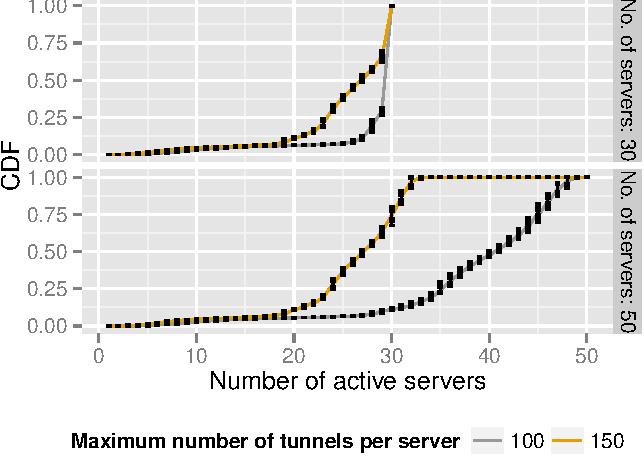
\includegraphics[width=1.0\columnwidth]{figures/instanceuse-multiserver-real.pdf}
  \caption{Impact of the maximum number of tunnels and servers on number of active servers in the virtual \gls{GGSN} model.}
\label{fig:instance_use_virtual}
  \end{center}
\end{figure}
In \reffig{instance_use_virtual} the \gls{CDF} of the number of active servers for four different virtual \gls{GGSN} configurations is displayed.
We observe, that increasing the number of supported tunnels per server allows a larger percentage of servers to be shut down or used for other tasks. This demonstrates the capability to scale the virtualized model in two dimensions quite well.
\begin{figure}[htbp]
  \begin{center}
  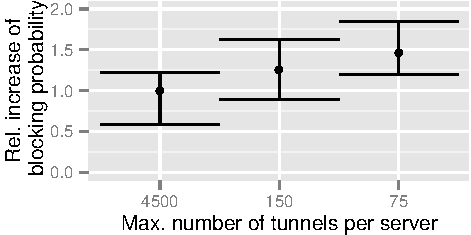
\includegraphics[width=1.0\columnwidth]{figures/blocking-comparison.pdf}
  \caption{Relative increase of blocking probability compared to the traditional \gls{GGSN}; $4500$ maximum tunnels per server being on a single server, $150$ on $30$, and $75$ on $60$ servers.}
\label{fig:blocking-comparison}
  \end{center}
\end{figure}
Next, we take a look at the blocking probability of the virtual \gls{GGSN} system in \reffig{blocking-comparison} and compare it to the results from the traditional \gls{GGSN} model dimensioned for $4500$ concurrent tunnels. We observe that
%, with the start up and shut down time of $5$ minutes in mind, 
the blocking probability increases by a factor of $1.48$ --- albeit at a still very low absolute scale ---  if the capacity of each server is set to $75$, i.e. \nicefrac{1}{60} of the original server capacity, while $27$ of all $60$ servers can be turned of or used for other purposes at $50\%$ of the time. We conclude, that choosing more powerful servers decreases the blocking probability but reduces the potential to disable servers.

\subsection{Impact of startup and shutdown times}
\label{sec:real_virtual_ggsn}
%So far we have considered a conservative start up and shut down time of servers of 5 minutes, which can potentially occur if current generation physical servers are used.
In this section, we first consider the impact of different boot and shut down times, for example if fast flash storage is used, on resource utilization and blocking probabilities. Afterwards, the influence of varying server start and stop times on a fixed combination of maximum tunnels and servers in the system is examined.
\begin{figure*}[htb]
  \begin{center}
  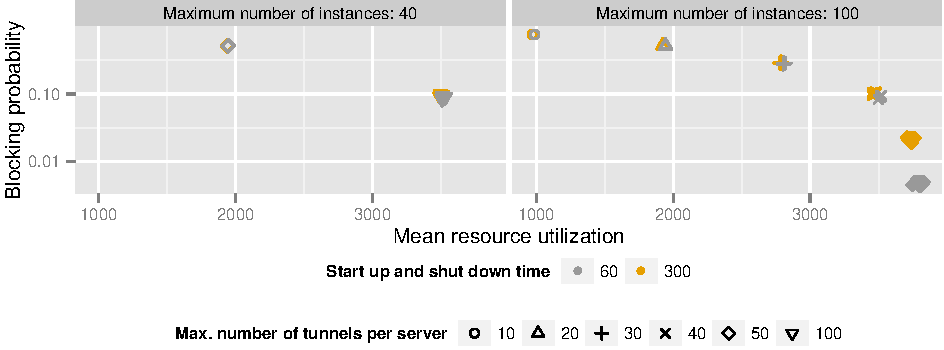
\includegraphics[width=1.0\textwidth]{figures/compare-util-block.pdf}
  \caption{Trade-off between blocking probability and mean resource utilization with regard to maximum number of servers, maximum number of tunnels per server, and start up and shut down time.}
 \label{fig:compare_util_block}
  \end{center}
\end{figure*}
\reffig{compare_util_block} shows scenarios with $40$ and $100$ number of virtual \gls{GGSN} instances surmounting to a total tunnel capacity between $1000$ to $5000$.
We study the impact of selecting different tunnel capacities per virtual instance as well as start up and shut down times on the blocking probability and mean resource utilization.
We observe that by increasing the number of servers, i.e., scaling out, the blocking probability can be decreased, while maintaining a relatively low mean resource utilization.
In addition to the previous effects, we notice that a higher start up and shut down time causes a slight increase in blocking probability for servers with low tunnel capacity.
\begin{figure}[htbp]
  \begin{center}
  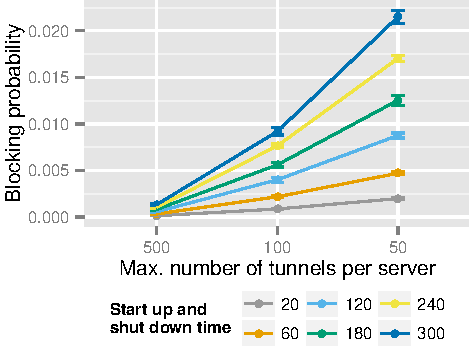
\includegraphics[width=1.0\columnwidth]{figures/compare-maxinstances-block.pdf}
  \caption{Influence of start up and shut down time on blocking probability with regard to different numbers of servers.}
  \label{fig:compare_maxinstances_block}
  \end{center}
\end{figure}
To study this behavior in more detail, we focus on a specific scenario in \reffig{compare_maxinstances_block}, where $5000$ total tunnels should be supported by the system.
In order to achieve this goal, we consider three types of instances, with the server capacity varying between $50$ and $500$. In each case we change the start up and shut down time between $1$ and $5$ minutes.
Lower server capacities combined with higher start up and shut down times increase the blocking probability. This is can in part be attributed to the simplistic instance start up threshold mechanism used in the model, which does not take the additional capacity gained by activating an additional server into account. 
%If a low capacity server with a long boot time is activated, there is a high probability that the system will quickly exhaust its capacity again.
If smaller instances are to be used, for example because they are cheaper than large instances, start up delay should be kept minimal or an appropriate instance management strategy has to be chosen.

